\documentclass[a4paper,12pt]{article}
\usepackage{fullpage}
\usepackage{ucs}
\usepackage{natbib}
\usepackage{graphicx}
\bibliographystyle{apalike}
\author{Willem E. Saris\\Daniel Oberski\\ESADE, Universitat Ramon Llull\\\\Jacques Hagenaars\\Tilburg University}

\title{Categorisation errors and differences in the quality of questions across countries}


\begin{document}
\maketitle
\begin{abstract}
The European Social Survey (ESS) has the unique characteristic that in more than 20 countries the same questions are asked and that within each round of the ESS Multitrait-Multimethod (MTMM) experiments are built in to evaluate the quality of a limited number of questions. This gives us an exceptional opportunity to observe the differences in quality of questions over a large number of countries. The MTMM experiments make it possible to estimate the reliability, validity and method effects of single questions \citep{andrews_construct_1984,saris_new_2004,saris_evaluation_1991}. The product of the reliability and the validity can be interpreted as the explained variance in the observed variable by the variable one would like to measure. It is a measure of the total quality of a question.

These MTMM experiments showed that there are considerable differences in measurement quality across countries. Because these differences in quality can cause wrong conclusions with respect to differences in relationships across countries this paper studies several reasons for these differences.
\end{abstract}\newpage

\section*{Introduction}

Measurement error can invalidate conclusions drawn from cross-country comparisons if the errors differ from country to country \citep{Saris_design_2007}. For this reason, when different groups such as countries as compared with one another, attention should not only be given to absolute levels of errors, but also to the differences between the groups. Different strategies have been developed to deal with the problem, for example within the context of invariance testing in the social sciences \citep{joreskog_simultaneous_1971}, differential item function in psychology \citep{muthen_multiple_1985}, and differential measurement error models in epidemiology and biostatistics \citep{carroll_nonlinear_1995}.

In the ESS a lot of time, money, and effort is spent to make the questions as functionally equivalent across countries as possible \citep{harkness_cross-cultural_2002} and to make the samples as comparable as possible \citep{hader_2007}\nocite{jowell_measuring_2007}. Nevertheless, considerable differences in quality of the questions can be observed across countries (see Table \ref{tab:countries}). In round 2 of the ESS the largest difference found was between questions in Sweden with a quality of .4 and in Portugal with a quality above .9. The Scandinavian countries had an average quality around .5 over 54 questions while other countries such as Greece, Portugal and Estonia had an average quality of .8.  To study these differences is important because these differences can cause differences in relationships between variables in different countries which have no substantive meaning but are just caused by differences in quality in the measurement \citep{Saris_design_2007}. In order to avoid such differences it is also important to study reasons for these differences in quality. 

In an earlier study, we investigated differences in translations, differences in the experiments' design, and differences in the complexity of the question as possible reasons for differences in question quality across countries \citep{oberski_differences_}. Here we consider differences in categorisation errors or use of the answer scale as a source of differences between countries. 

First we provide the necessary background: the response model we use as our starting point, and explanations of the multitrait-multimethod (MTMM) experiments we use to assess question quality  and of categorisation error. Next we give a short overview of our limited previous findings on the origins of cross-country differences in measurement error. We then present the data from the European Social Survey and the structure of the experiments, and discuss the methods used to analyse these data. The subsequent section describes our analysis of categorisation errors for four experiments using categorical scales, and ends with a meta-analysis of these results. We then summarise and discuss our findings. Finally, some general conclusions are drawn and suggestions for further research are indicated.

\section{Background}

In Figure \ref{fig:response} we show the basic response model \citep{Saris_design_2007} we use as our starting point. 

\begin{figure}[htb]
\centering
%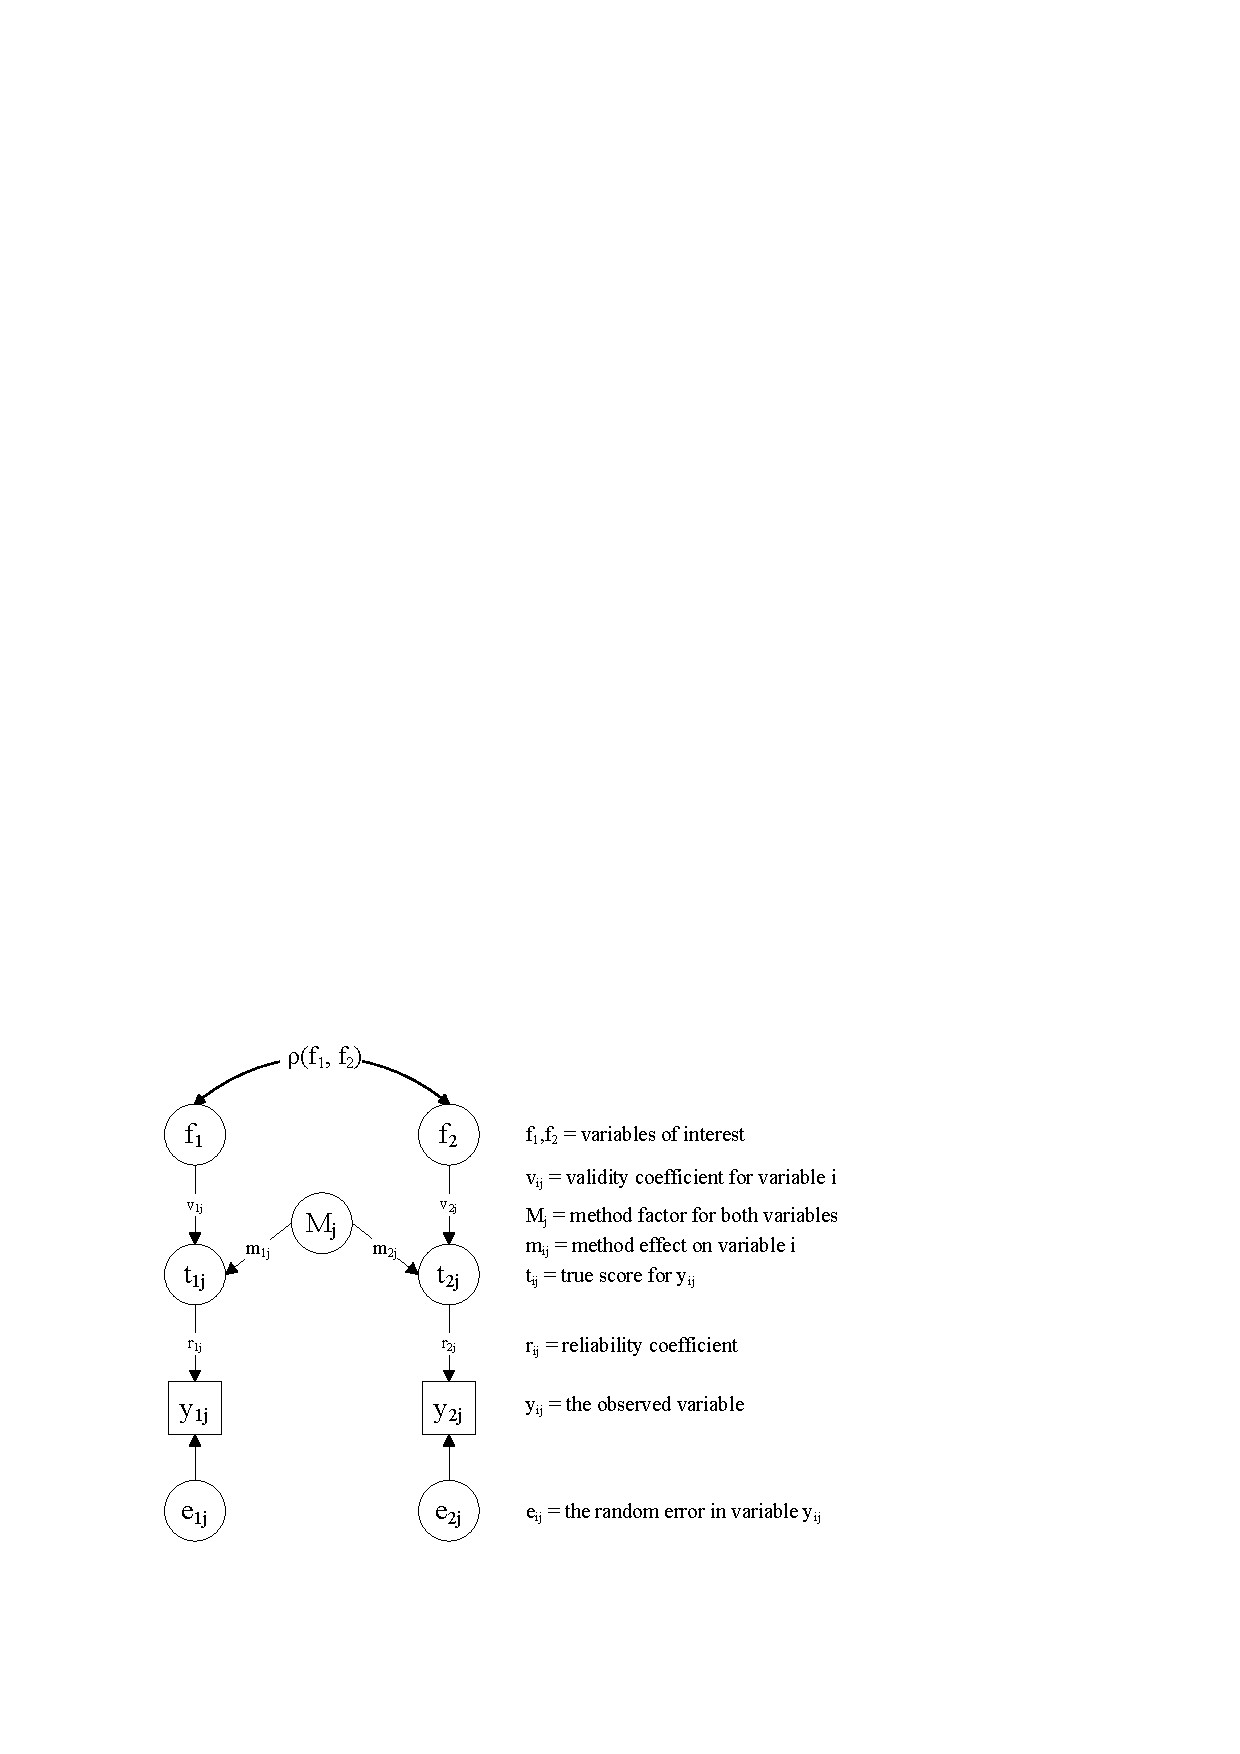
\includegraphics[width=.7\textwidth]{response_model}
\caption{The response model used in the MTMM experiments.\label{fig:response}}
\end{figure}

The difference between the observed response ($y$) and the so called `true score' ($t$) is random measurement error ($e$). So the coefficient $r$ represents the reliability coefficient and $r^2$ is the reliability.
The difference between the true score and the concept by intuition ($f_1$) are the respondents' systematic reactions to the method ($m$). So the coefficient $v$ represents the true score validity coefficient and $v^2$ is the true score validity. The quality of a measure ($q^2$) is defined as  $q^2 =  r^2 . v^2$ and $q$ is the quality coefficient. This quality--sometimes also called the reliability ratio--equals $\frac{Var(f)}{Var(y)}$: it can be interpreted as the proportion of variation in the observed variable that is due to the unobserved trait of interest. The correlation between the unobserved variables of interest is denoted by $\rho(f_1,f_2)$.

Several remarks should be made. The first is that the correlation $\rho(y_i, y_j)$ between two observed variables is:
\begin{equation}
\rho(y_i, y_j) = \overbrace{\rho(f_i, f_j)}^{\textrm{Correlation of interest}} \cdot \overbrace{q_i \cdot q_j}^{\textrm{Attenuation factor}} + \overbrace{r_i \cdot r_j \cdot m_i \cdot m_j}^{\textrm{Correlation due to method}}
\label{eqn:attenuation}\end{equation}
This means that the correlation between the observed variables is normally smaller than the correlation between the variables of interest, but can be larger if the method effects are considerable. A second remark to make is that one can not compare correlations across countries without correction for measurement error if the measurement quality coefficients are very different across countries: this follows directly from the above equation (\ref{eqn:attenuation}). A third point is that one can not estimate these quality indicators from this simple design with two observed variables. In this model there are two reliability coefficients, two validity coefficients, two method effects and one correlation between the two latent traits, leaving us with seven unknown parameters, while only one correlation can be obtained from the data. It is impossible to estimate these seven parameters from just one correlation.  

There are two different approaches to estimate these coefficients. The first is the use of MTMM experiments. The second is the use of the prediction program SQP that is based on a large number of MTMM experiments \citep{oberski_sqp_}. Because we use the MTMM approach here, it is briefly introduced below. A more elaborate introduction to MTMM and SQP can be found in Saris and Gallhofer (2007).

\subsection{MTMM models}

Campbell and Fiske (1959) suggested using multiple traits and multiple methods (MTMM). The classical MTMM approach recommends the use of a minimum of three traits that are measured with three different methods leading to nine different observed variables. An example of such a design is given in Table \ref{tab:design}.  

\begin{table}[htb]\caption{The classic MTMM design used in the ESS pilot study.\label{tab:design}}
\fbox{\begin{minipage}{\textwidth}
The three traits were presented by the following three requests:
\begin{itemize}
\item \textit{On the whole, how satisfied are you with the present state of the economy in Britain?}
\item \textit{Now think about the national government. How satisfied are you with the way it is doing its job?}
\item \textit{And on the whole, how satisfied are you with the way democracy works in Britain?} 
\end{itemize}

The three methods are specified by the following response scales: 
\begin{quote}
\textit{(1) Very satisfied; (2) Fairly satisfied; (3) Fairly dissatisfied; (4) Very dissatisfied}  
\begin{tabular}{ccccccccccc}
\textit{Very dissatisfied		}&&&&&&&&&&			        \textit{Very satisfied}\\
		       0 &    1&     2 &    3&     4     &5     &6     &7     &8     &9     &10\\
\end{tabular}

\textit{(1) Not at all satisfied; (2) Satisfied;  (3) Rather satisfied;  (4) Very satisfied}
\end{quote}\end{minipage}}
\end{table}


\begin{figure}[htb]\centering
%\includegraphics[width=.7\textwidth]{mtmm}
\caption{\label{fig:mtmm}MTMM model illustrating the true scores and their factors of interest.}
\end{figure}

Collecting data using this MTMM design, data for nine variables are obtained and from that data a correlation matrix of $9 \times 9$ is obtained. The model formulated to estimate the reliability, validity, and method effects is an extension of the model presented in Figure \ref{fig:response}. This figure illustrates the relationships between the true scores and their general factors of interest. Figure \ref{fig:mtmm} shows that each trait ($f_i$) is measured in three ways. It is assumed that the traits are correlated but that the method factors ($M_1$, $M_2$, $M_3$) are not correlated. To reduce the complexity of the figure, it is not indicated that for each true score there is an observed response variable that is affected by the true score and a random error as was previously introduced in the model in Figure \ref{fig:response}. However, these relationships, although not made explicit, are implied.  

The MTMM design of 3 traits and 3 methods generates 45 covariances and variances. In turn, these 45 pieces of information provide sufficient information to estimate 9 reliability and 9 validity coefficients, 3 method effect coefficients and 3 correlations between the traits. In total there are 24 parameters to be estimated. This leaves $45 - 24 = 21$ degrees of freedom, meaning that the necessary condition for identification is fulfilled. It also can be shown that the sufficient condition for identification is satisfied and given that $df=21$ a test of the model is possible.

Table \ref{tab:mtmm_cor} presents the correlations that we derived between the 9 measures obtained from a sample of 481 people in the British population. Using the specifications of the model indicated above and the ML estimator to estimate the quality indicators, the results presented in Table \ref{tab:mtmm_results} are obtained\footnote{In this case the ML estimator is used. The estimation is done using the covariance matrix as the input matrix and not the correlation matrix . Thereafter, the estimates are standardized to obtain the requested coefficients. A result of this is that the standardized  method effects are not exactly equal to each other.}.  

\begin{table}[htb]\centering\caption{Correlations between nine measures obtained from a sample of 481 people from the British population. Correlations between a repetition of a trait using a different method (`monotrait-heteromethod' correlations) are indicated in boldface.\label{tab:mtmm_cor}}
\begin{tabular}{lrrrrrrrrr}\hline
& \multicolumn{3}{c}{Method 1} & \multicolumn{3}{c}{Method 2} & \multicolumn{3}{c}{Method  3} \\ 
\hline
& Q1 & Q2 & Q3 & Q1 & Q2 & Q3 & Q1 & Q2 & Q3 \\ 
Method 1\\ 
Q1 & 1.00 \\ 
Q2 & .481 & 1.00 &  \\ 
Q3 & .373 & .552 & 1.00 \\ 
Method 2\\ 
Q1 & \textbf{-.626} & -.422 & -.410 & 1.00 \\ 
Q2 & -.429 & \textbf{-.663} & -.532 & .642 & 1.00 \\ 
Q3 & -.453 & -.495 & -\textbf{.669} & .612 & .693 & 1.00 \\ 
Method 3\\
Q1 & -\textbf{.502} & -.374 & -.332 & .\textbf{584} & .436 & .438 & 1.00 \\ 
Q2 & -.370 & -\textbf{.608} & -.399 & .429 & .\textbf{653} & .466 & .556 & 1.00 \\ 
Q3 & -.336 & -.406 & -\textbf{.566} & .406 & .471 & .\textbf{638} & .514 & .558 & 1.00 \\ 
 \\ 
Mean & 2.42 & 2.71 & 2.45 & 5.26 & 4.37 & 5.13 & 2.01 & 1.75 & 2.01 \\ 
Standard Deviation & .77 & .76 & .84 & 2.29 & 2.37 & 2.44 & .72 & .71 & .77 \\ 
\hline
\end{tabular}
\end{table}

\begin{table}[htb]\centering\caption{The standardised estimates of the MTMM parameters (figure \ref{fig:mtmm}), which are obtained when analysing the sample covariance matrix above.\label{tab:mtmm_results}}
\begin{tabular}{lrrrrrrrr}\hline
 &   \multicolumn{3}{c}{Validity coeffs} & \multicolumn{3}{c}{Method effects} &  & Reliability coeff.\\ 
 \hline
    & F1 & F2 & F3 & M1 & M2 & M3 \\ 
T11   & .93 &  &  & .36 &  &  &  & .79 \\ 
T21   &  & .94 &  & .35 &  &  &  & .85 \\ 
T31   &  &  & .95 & .33 &  &  &  & .81 \\ 
 \\ 
T12   & .91 &  &  &  & .41 &  &  & .91 \\ 
T22   &  & .92 &  &  & .39 &  &  & .94     \\ 
T32   &  &  & .93 &  & .38 &  &  & .93 \\ 
 \\ 
T13   & .85 &  &  &  &  & .52 &  & .82 \\ 
T23   &  & .87 &  &  &  & .50 &  & .87\\ 
T33   &  &  & .88 &  &  & .48 &  & .84  \\
\hline
\end{tabular}
\end{table}
\hfill
\subsection{The categorical response model}

The response model discussed so far makes no mention of the fact that many of the measures we use are in fact ordinal--that is, they are ordered categories rather than measured on a continuous scale. 
Broadly speaking, two types of measurement models have been proposed for this situation. The first assumes there is an unobserved categorical variable, and that errors arise from the conditional chances of choosing a category on the survey question given the unobserved score. Such models are often referred to as latent class models \citep{lazarsfeld_latent_1968,hagenaars_applied_2002}.

The second approach deals with the case where a continuous scale or `latent response variable' is thought to underly the observed categorical item. Such models are sometimes called latent trait models. Several possible extensions are possible, but we focus on a special case described by \citet{muthen_general_1984}. This is the model we will use in our subsequent analysis of the data\footnote{It can be shown that analysing polychoric correlations in an MTMM model is a special case of the model we use \citep{muthen_latent_2002}. However, we do not use polychoric correlations because it would be  necessary to assume that the variances of the latent response variables are equal across countries. Since we try to separate categorisation errors from differences in the continuous part of the model, this is not a desirable assumption. The model we use is equivalent to a multi-dimensional two parameter graded response model in item response theory \citep{muthen_latent_2002}.}.

Errors may arise at two stages. The first is the connection between the latent response variable and its latent trait. This part of the error model is completely analagous to factor analysis or MTMM models for continuous data: the scale is modelled as a linear combination of a latent trait, a reaction to the particular method used to measure the trait, and a random error, and interest then focuses on the connection between the trait and the scale, which we again term the `quality coefficient' (see figures \ref{fig:response} and \ref{fig:mtmm}). It should be noted that, because we are interested only in the quality coefficient and not in the separation of the reliability and validity coefficients, we do not make a distinction between the true score and the latent trait as is done in the true score model explained above. The true score and classic MTMM models are, however, equivalent \citep{coenders_testing_2000}.

The second stage at which errors arise differs from the continuous case. Here the continuous latent response variable is split up into the different categories, such that each category of the observed variable corresponds to a certain range on the unobserved continuous scale. The sizes of these ranges are determined by threshold parameters. Several types of errors can be distinguished at this stage \citep{coenders_structural_1996}:
\begin{enumerate}
\item \emph{Grouping errors} occur because the infinite possible values of the latent response variable are collapsed into a fixed number of categories. These errors will be higher when there are fewer categories;
\item \emph{Transformation errors} occur when the distances between the numerical scores assigned to each category are not the same as the distances between the means of the latent response variable in those categories. This happens when the thresholds are not equally spaced, or when the available categories do not cover the unobserved opinions adequately. 
\end{enumerate}
Categorisation, then, can be expected to be another source of measurement error besides random errors and method variance. If these errors differ across countries, then so will the overall measurement quality, and differences in means, correlations, regression coefficients, and cross-tables across countries result which are due purely to differences in measurement errors.

The model we use allows to a certain extent for the separation of errors due to the categorisation, errors due to the reaction to the method and random errors. In this paper we take advantage of this separation to compare the amount of error due to categorisation introduced across countries. 

\subsection{Categorisation errors in survey questions}

The previous sections showed that, using the MTMM design, it is possible to obtain a measure ($q^2$) of the total quality of a question. If a continuous model is used, this quality is influenced by errors in both stages of the categorical response model: not only random errors and method effects are included, but also errors due to the categorisation. Consequently the linear MTMM model assuming continuous variables does not discount categorisation errors, but includes them to a certain extent in the estimates of the quality and other parameters \citep{coenders_structural_1996}.

However, since the quality coefficient is estimated from the covariance matrix of the measures, it can be both reduced and increased by categorisation errors. In general all correlations between measures increase after correction for categorisation, but they need not all increase equally. For example, consider again table \ref{tab:mtmm_cor}. If categorisation errors are higher using the first method then the correlations between the latent response variables using this method (the upper-left triangle of the matrix) will increase more relative to the observed correlations than the correlations of each variable with its repetition using a different method (in bold). In this case the amount of variance in the reponse variable due to the method will be larger in the categorical model than in the continuous model, and the estimated quality of the measure in the categorical response model can become lower than the estimated quality in the continuous MTMM model. This is because there are method effects (correlated errors) on the level of the continuous latent response variables which do not manifest themselves in the observed (Pearson) correlations between the categorical variables. Categorisation can therefore in some cases inflate estimates of the quality of categorical observed variables, even though, at the same time, it causes errors which reduce the quality. There are thus two processes at work, which have opposite effects on the estimates of the quality.

Because it can both reduce and artificially inflate estimates of quality, categorisation error is an important possible cause of finding differences in question quality across countries. If either of these two processes differs from one country to another, the estimates of the quality can be expected to differ as well. Therefore, we focus here on the changes in the quality coefficient one observes in a continuous reponse model relative to a categorical model. This allows us to study the attentuation or inflation of quality estimates across countries.

As noted before, the quality (or reliability ratio) of a variable is defined as the ratio of the true trait variance to the observed variance (see also figure \ref{fig:response} in the first section):
\begin{equation}
q^2 = \frac{Var(f)}{Var(y)}.\label{eqn:relratio}
\end{equation}
However, we have now seen that $y$ is itself a categorization of an unobserved continuous variable ($c$), and therefore the above equation \ref{eqn:relratio} can be `decomposed' into
\begin{equation}
q^2 =  \frac{ Var(f)}{Var(c)} \cdot \frac{Var(c)}{Var(y)}.		
\end{equation}
The scale of $c$ is arbitrary, except that it may vary across countries due to relative differences in variance (Muth\'en \& Asparouhov, 2002). However, the ratio $Var(c)/Var(y)$ can easily be calculated once $q^2$, the quality from the continuous analyis, and $Var(f)/Var(c)$, the quality from the categorical MTMM analysis, have been obtained. So the effect of categorisation on the quality estimate can be derived. We attach no specific significance to this number other than that it is a useful index of the relative differences between the quality estimates of the continuous and categorical models.

In the present study, we estimate this `categorisation factor' for different countries and experiments, and examine to what extent it can explain the differences in quality across countries. First, however, we give an overview of the data we use.


\section{Data}

The European Social Survey (ESS) has the unique characteristic that in more than 20 countries the same questions were asked and that within each round of the ESS Multitrait-Multimethod (MTMM) experiments are built in to evaluate the quality of a limited number of questions. This gives us an exceptional opportunity to observe the differences in quality of questions over a large number of countries. In this paper we have used the MTMM experiments of round 2 of the ESS. The topics of the 6 MTMM experiments in the second round of the ESS were the following:
\begin{enumerate}
\item Time spent on housework;
\item The social distance between the doctor and patients;
\item Opinions about job;
\item The role of men and women in society;
\item Satisfaction with the political situation;
\item Political trust.
\end{enumerate}
Concerning each of these topics 3 questions were asked and these three questions were presented in 3 different forms following the discussed MTMM designs 
\citep{campbell_convergent_1959}. The first form,  used for all respondents, was presented in the main questionnaire. The two alternative forms were presented in a supplementary questionnaire which was completed after the main questionnaire. All respondents were only asked to reply to one alternative form but different groups got different version of the same questions \citep{saris_new_2004}. For the specific questions for the 6 experiments we refer to the ESS website where the English source version of all questions are presented\footnote{http://www.europeansocialsurvey.org}, and for the different translations we refer to the ESS archive\footnote{http://ess.nsd.uib.no}.

	Each experiment varies a different aspect of the method by which questions can be asked in questionnaires. The `housework' experiment compares numeric estimates by respondents with other scales. The `doctors' experiment examines the effect of choosing arbitrary scale positions as a starting point for agreement-disagreement with a statement. The `job' experiment compares a 4 point with an 11 point scale and a true-false scale with a direct question. In the `women' experiment agree-disagree scales are reversed, there is one negative item, and a `don't know' category is omitted in one of the methods.  The `satisfaction' experiment varies the extremeness and number of fixed reference points of the scale. And finally, the experiment on political trust was meant to investigate the effect of repeating the same question in the same format.

A special group took care that the samples in the different countries where proper probability samples and as comparable as possible \citep{hader_2007}. 

The questions asked in the different countries have been translated from the English source questionnaire. An optimal effort has been made to make these questions as equivalent as possible and to avoid errors. In order to reach this goal two translators independently translated the source questionnaire and a third person was involved to choose the optimal translation by consensus if differences were found. For details of this procedure we refer to the work of \citet{harkness_cross-cultural_2002}.

	 Despite these efforts to make the data as comparable as possible, large differences in measurement quality were found across the different countries.  Table \ref{tab:countries} shows the mean and median standardised quality of the questions in the main questionnaire across the experiments for the different countries.

\begin{table}[hbt]\centering\caption{The quality of all 18 questions included in the experiments in the main questionnaire.\label{tab:countries}}
\begin{tabular}{lrrrr}
\hline
Country&Mean&Median&Minimum&Maximum\\\hline
Portugal&0.79&0.81&0.63&0.91\\
Switzerland&0.79&0.84&0.56&0.90\\
Greece&0.78&0.79&0.64&0.90\\
Estonia&0.78&0.85&0.58&0.90\\
Poland&0.73&0.85&0.51&0.90\\
Luxembourg&0.72&0.73&0.53&0.88\\
United Kingdom&0.70&0.71&0.56&0.82\\
Denmark&0.70&0.70&0.52&0.80\\
Belgium&0.70&0.73&0.46&0.90\\
Germany&0.69&0.70&0.53&0.83\\
Spain&0.69&0.64&0.54&0.90\\
Austria&0.68&0.68&0.51&0.85\\
Czech Republic&0.65&0.60&0.52&0.87\\
Slovenia&0.63&0.60&0.46&0.82\\
Norway&0.59&0.59&0.35&0.83\\
Sweden&0.58&0.58&0.43&0.68\\
Finland&0.57&0.54&0.42&0.78\\
	\hline
\end{tabular}
\end{table}

A remarkable phenomenon in this table is that the Scandinavian countries have the lowest quality of all while the highest quality has been obtained in Portugal, Switzerland, Greece, and Estonia. The other countries are in between these two groups. 
The differences are considerable and statistically significant across countries ($F=3.19$, $df=16$, $p<.001$) and experiments ($F=92.65$, $df=5$, $p<.0001$)\footnote{The significance of the differences in the quality coefficients was determined using their observed distribution.}. The highest mean quality is .79 in Portugal while the lowest is .57 in Finland. If the correlation between the constructs of interest is .6 in both countries and the measures for these variables have the above quality then the observed correlation in Portugal would be .474 while the observed correlation in Finland would be .342. Most people would say that this is a large difference in correlations which requires a substantive explanation. But this difference can be expected because of differences in data quality and has no substantive meaning at all.

\section{Explanations for cross-country differences in question quality}

The previous section showed that in some cases large differences were found in question quality across the countries of the ESS. In a previous study, we examined a few possible explanations of these discrepancies \citep{oberski_differences_}.

The first explanation we studied were errors in the translation. Although in the ESS a lot of care has been taken to ensure the correct translation of the questions, we found that a few questions in the supplementary questionnaire had not been translated as intended. In particular, one item in the `doctors' experiment had been translated in all French questionnaires as `Doctors rarely tell their patients the whole truth' rather than `Doctors rarely keep the whole truth from their patients'. Since these sentences have opposite meanings, it is unsurprising that we should find a different relationship with the trait of interest.

Another alternative explanation for differences across countries is differences in the implementation of the experimental design. Here one difference existed between the implementations in Norway, Sweden, and Finland and the other countries: in these countries respondents could send in the supplementary questionnaire containing the repetitions at a time chosen by themselves, while the general design used in other countries was that the supplementary questionnaire was administered directly after the main interview. Since in some cases quite some time passed before the second questionnaire was completed, it is possible that the opinion has in this time changed or that other unique considerations are taken into account at the second moment than at the first moment. An MTMM analysis of a sample split according to whether the questionnaire was returned within two days or later provided strong evidence that this was indeed the case. In fact, the sample which returned the questionnaire on the same day by itself was very similar with respect to the quality to other countries. 

The third alternative we considered was that the language of the questions could be more complex in one language than in another. Previous meta-analyses found that language complexity can have an effect on the quality \citep{saris_estimation_2007}. However, we found no strong evidence that the complexity of the questions caused differences in question quality in this case.

Thus, in some cases we found artificial differences in quality which are likely to be due to an erroneous translation or different implementation of the experimental design--notably in the Scandivian countries except Denmark and for one item in the French-speaking countries. However, these cases are not so numerous that they can explain the large overall variations in question quality that were found in the ESS. Therefore we now turn to the possibility that the use of the categories in the categorical questions differs from country to country, and proceed to investigate the influence of categorisation errors on the quality in different countries and experiments.

\section{Methods}

...

The estimation was done using the weighted least squares approach described by \citet{flora_empirical_2004}.

There is a simple relationship between the threshold and quality coefficients of our model and difficulty and discrimination parameters in IRT models: the quality coefficients are scaled discrimination parameters, while a scaled difficulty for each category can be obtained by dividing each threshold by the corresponding quality coefficient \citep{muthen_latent_2002}.

\section{Results}

We estimated the quality of the measures based on the continuous model and based on the categorical model for four experiments which used an answer scale of five categories or less in the main questionnaire. For each of these questions we took the ratio of the two different quality measures as an index of the effect that categorisation has on the continuous quality estimates. The first experiment's results will be described in some detail, while we provide the results of the other experiments more briefly.

\subsection{Experiment 1}

The first experiment concerned opinions on the role of women in society (see table \ref{card:women}). We first turn to the hypothesis that all thresholds are equal across different countries. If this hypothesis cannot be rejected then there is also little reason to think that the categorisation is causing differences in the quality coefficients. 

We selected the two countries with the highest and the country with the lowest quality coefficients. In this experiment, the wording of the question reversed in the second method. For example, the statement `When jobs are scarce, men should have more right to a job than women' from the main questionnaire was changed to `When jobs are scarce, women should have the same right to a job as men' in the supplementary questionnaire. The countries with high quality coefficients were, in this case, Portugal and Greece. The lowest coefficients for this experiment were found in Estonia. To be able to separately study misspecifications in the categorisation part of the model, we imposed no restrictions on the covariance matrix of the latent response variables at this stage. 

\begin{table}\caption{\label{card:women}The `women' experiment: questions and threshold estimates (in z-scores).}\fbox{\begin{minipage}{\textwidth}\begin{small}
%	

`A woman should be prepared to cut down on her paid work for the sake of her family'

 \begin{scriptsize}\begin{tabular*}{\textwidth}{lp{.12\textwidth} lp{.12\textwidth}cp{.12\textwidth}cp{.12\textwidth}cp{.12\textwidth}cp{.12\textwidth} }
 &  \parbox{.10\textwidth}{\centering 1} & $\tau_1$ &  \parbox{.10\textwidth}{\centering 2} & $\tau_2$ &  \parbox{.10\textwidth}{\centering 3} & $\tau_3$ &  \parbox{.10\textwidth}{\centering 4} & $\tau_4$ &  \parbox{.10\textwidth}{\centering 5}\\
 &\parbox{.12\textwidth}{\centering \textit{Agree strongly}} & &\parbox{.12\textwidth}{\centering \textit{Agree}} && \parbox{.12\textwidth}{\centering \textit{Neither disagree nor agree}} && \parbox{.12\textwidth}{\centering \textit{Disagree}} && \parbox{.12\textwidth}{\centering \textit{Disagree strongly}} \\
  Slovenia && -1.4 && -0.1 && 0.6 && 1.8 \\
 Greece && -1.1 && -0.2 && 0.5 && 1.4 \\
 \end{tabular*}\end{scriptsize}

\vspace{12pt}

`A woman should not have to cut down on her paid work for the sake of her family.'

 \begin{scriptsize}\begin{tabular*}{\textwidth}{lp{.12\textwidth} lp{.12\textwidth}cp{.12\textwidth}cp{.12\textwidth}cp{.12\textwidth}cp{.12\textwidth} }
 &  \parbox{.10\textwidth}{\centering 1} & $\tau_1$ &  \parbox{.10\textwidth}{\centering 2} & $\tau_2$ &  \parbox{.10\textwidth}{\centering 3} & $\tau_3$ &  \parbox{.10\textwidth}{\centering 4} & $\tau_4$ &  \parbox{.10\textwidth}{\centering 5}\\
  Slovenia && -1.5 && -0.0 && 0.6 && 2.0 \\
 Greece && -1.5 && -0.3 && 0.4 && 1.5 \\
 \end{tabular*}\end{scriptsize}

\vspace{12pt}

`Men should take as much responsibility as women for the home and children.'

 \begin{scriptsize}\begin{tabular*}{\textwidth}{lp{.12\textwidth} lp{.12\textwidth}cp{.12\textwidth}cp{.12\textwidth}cp{.12\textwidth}cp{.12\textwidth} }
 &  \parbox{.10\textwidth}{\centering 1} & $\tau_1$ &  \parbox{.10\textwidth}{\centering 2} & $\tau_2$ &  \parbox{.10\textwidth}{\centering 3} & $\tau_3$ &  \parbox{.10\textwidth}{\centering 4} & $\tau_4$ &  \parbox{.10\textwidth}{\centering 5}\\
  Slovenia && -0.5 && 1.3 && 1.9 && 2.6 \\
 Greece && -0.6 && 0.7 && 1.6 && 2.3 \\
 \end{tabular*}\end{scriptsize}

\vspace{12pt}

`Women should take more responsibility for the home and children than men'

 \begin{scriptsize}\begin{tabular*}{\textwidth}{lp{.12\textwidth} lp{.12\textwidth}cp{.12\textwidth}cp{.12\textwidth}cp{.12\textwidth}cp{.12\textwidth} }
 &  \parbox{.10\textwidth}{\centering 1} & $\tau_1$ &  \parbox{.10\textwidth}{\centering 2} & $\tau_2$ &  \parbox{.10\textwidth}{\centering 3} & $\tau_3$ &  \parbox{.10\textwidth}{\centering 4} & $\tau_4$ &  \parbox{.10\textwidth}{\centering 5}\\
  Slovenia && -1.7 && -0.7 && -0.2 && 1.2 \\
 Greece && -1.6 && -0.5 && 0.0 && 1.4 \\
 \end{tabular*}\end{scriptsize}

\vspace{12pt}

`When jobs are scarce, men should have more right to a job than women.'

 \begin{scriptsize}\begin{tabular*}{\textwidth}{lp{.12\textwidth} lp{.12\textwidth}cp{.12\textwidth}cp{.12\textwidth}cp{.12\textwidth}cp{.12\textwidth} }
 &  \parbox{.10\textwidth}{\centering 1} & $\tau_1$ &  \parbox{.10\textwidth}{\centering 2} & $\tau_2$ &  \parbox{.10\textwidth}{\centering 3} & $\tau_3$ &  \parbox{.10\textwidth}{\centering 4} & $\tau_4$ &  \parbox{.10\textwidth}{\centering 5}\\
  Slovenia && -1.8 && -0.8 && -0.3 && 0.9 \\
 Greece && -0.9 && 0.1 && 0.6 && 1.4 \\
 \end{tabular*}\end{scriptsize}

\vspace{12pt}

`When jobs are scarce, women should have the same right to a job as men.'

 \begin{scriptsize}\begin{tabular*}{\textwidth}{lp{.12\textwidth} lp{.12\textwidth}cp{.12\textwidth}cp{.12\textwidth}cp{.12\textwidth}cp{.12\textwidth} }
 &  \parbox{.10\textwidth}{\centering 1} & $\tau_1$ &  \parbox{.10\textwidth}{\centering 2} & $\tau_2$ &  \parbox{.10\textwidth}{\centering 3} & $\tau_3$ &  \parbox{.10\textwidth}{\centering 4} & $\tau_4$ &  \parbox{.10\textwidth}{\centering 5}\\
  Slovenia && -0.8 && 0.7 && 1.1 && 1.9 \\
 Greece && -1.1 && -0.1 && 0.7 && 2.0 \\
 \end{tabular*}\end{scriptsize}

\vspace{12pt}

\end{small}\end{minipage}}\end{table}

In the first analysis, all thresholds were constrained to be equal across the five countries. This yields a likelihood ratio statistic of 507 on 48 degrees of freedom. The country with the highest (128) contribution to this chi-square statistic is Portugal. When we examine the expected parameter changes, it also turns out that in this country these standardised values are very large with some values close to .9 while in other countries the highest obtained and exceptional value is .6. For some reason, the equality constraint on the Portuguese thresholds appears to be a particularly gross misspecification.

As it turns out, this particular misspecification is very likely due to a translation error. The intention of the experiment was to reverse the wording of the question in the second method. But in Portugal the reverse wording was not used, and the same version was presented as in the main questionnaire. The supplementary questions mean something else in Portugal and therefore it makes sense that the thresholds should differ from those found in the other countries. To prevent incomparability when the MTMM model is estimated, we omit Portugal from our further analyses and continue with four countries. We should note, however, that the resulting experiment does provide a good opportunity to examine the effect of a repetition on the threshold structure. In addition, our analysis of the measurement model has revealed an item that was incorrectly translated in the supplementary questionnaire but had (as far as we know) gone undetected so far.

Continuing our analysis with two countries, the model where all thresholds are constrained to be equal yields a likelihood ratio of 351 and 36 degrees of freedom ($p<.00001$). This model should therefore be rejected: the thresholds are significantly different across countries. 

We formulated a new model in which some thresholds were constrained to be equal, while others were freed to vary. However, we found that too many parameters were freed for Greece and some parameters could again be constrained to be equal: the expected parameter change which led us to free these parameters is an estimate, which need not equal the actual parameter change. For some thresholds the actual change was negligible (although still within a 95\% confidence interval for the expected change) and we constrained these four parameters again. The resulting model has an approximate likelihood ratio of 2.8 on 2 degrees of freedom ($p=.24$)\footnote{It is also possible to free more parameters and put no restrictions at all on the model. This might lead us to find differences between countries more easily, since the parameters are allowed to vary. However, we prefer to aid our estimation by imposing these restrictions: if they do not hold in the population, this leads us to be conservative in ascribing differences between countries to the categorisation.}. The resulting estimates of the threshold parameters are presented in table \ref{card:women}. These estimates have been expressed as z-scores in order to make them comparable.

Table \ref{card:women} presents three different traits, each asked in two different forms. The first form of each trait is the form asked in the main questionnaire, while the second form was asked in the supplementary questionnaire (the third form has been omitted for brevity). 

Looking at the first question, it can be seen that the endpoints are somewhat distant, especially in Slovenia: there the category `disagree strongly' is 1.8 standard deviations or more away from the mean, reducing the number of scale points that are available for some people. The remaining categories, however, are reasonably similar, not too far away from the distribution of the opinion, and not very unequally spaced.

The second form of the same question is similar to the first form in this respect, except that here both of the endpoints are rather distant in both countries, again reducing the number of scale points. As noted above, a reduction in scale points can be expected to increase grouping errors.

The second trait (`responsibility') presents a radically different picture. In both countries the `disagree' and `disagree strongly' categories are quite far away from the mean. This again reduces the number scale points, while, at the same time, the scale is cut off in this manner only from one side. This may be because of a strong skew in the distribution of the opinion. Large transformation errors can be expected. Moreover, in Slovenia this effect is much worse than in Greece: the category `neither disagree nor agree' is already 1.3 standard deviations or more away from the mean,  reducing the amount of information provided by this variable in Slovenia even further. Thus, the problem with this particular question may be that it is very hard not to agree with it, and more so in Slovenia than in Greece.

The second phrasing of this question is, perhaps, more polemic and seems to provide a better coverage of the prevailing opinions on women and men's responsibility for the home and children.

For the third and last trait--the right to a job--the most striking feature of the thresholds is that in Slovenia, the first three categories represent opinions below the mean, while in Greece only the first category does. Beyond this, it is difficult to say which scale might produce fewer categorisation errors. Surprising, however, is that the second form of the same question seems to produce much more comparable scales with respect to the thresholds than the first one.

The thresholds provide some insight into the nature of categorisation errors. However, the final quality of the measure depends also on other parameters of the categorical response model such as the quality coefficients and the error variances. Since the quality is a complex of different parameters, the discrepancy between the quality obtained in the categorical model and the quality in the continuous model is more informative on the effects of categorisation. As explained above, we operationalise this discrepancy by taking the ratio $q^2_{continuous} / q^2_{categorical} $. Table \ref{tab:women} contains the quality estimates under both models together with this categorisation factor for the three questions in the main questionnaire.

\begin{table}\centering\caption{Quality according to the continuous and categorical models, with categorisation factors for the experiment on opinions about the role of men and women in society.\label{tab:women}}\begin{tabular}{lllrrr}
\hline
 &  &  & \multicolumn{3}{c}{`Women'} \\
 &  &  & CutDown & Respnsib. & MenRight\\
\hline
\multicolumn{2}{l}{Continuous analysis}\\		   
 & $q^2$ & Greece & 0.71 & 0.66 & 0.71\\
 &  & Slovenia & 0.54 & 0.25 & 0.68\\
\multicolumn{2}{l}{Categorical analysis}   &  &  &  & \\
 & $q^2$ & Greece & 0.51 & 0.35 & 0.48\\
 &  & Slovenia & 0.69 & 0.29 & 0.65\\
 \multicolumn{2}{l}{Categorisation factor}   &  &  &  & \\
 &  & Greece & 1.4 & 1.9 & 1.5\\
 &  & Slovenia & 0.8 & 0.9 & 1.0\\
\hline
\end{tabular}\end{table}

The top two rows of table \ref{tab:women} show that the quality in Greece was higher than in Slovenia using the continuous model; this is, indeed, the reason we chose these particular countries to compare. The quality in Slovenia is lower for the first question, dramatically lower for the second question, and very similar for the third question. This is in principle in line with the descriptions given above of our expectations of categorisation errors.

However, table \ref{tab:women} also shows that such interpretations of the possible influence of the thresholds are not as straightforward as they might seem. We fitted the MTMM model to the estimated covariance matrix of the latent response variables, and obtained a model which seemed to fit reasonably well ($\chi^2 = 20$, $df=10$, $p=.02$). While for the first and second questions the low qualities are indeed corrected upwards somewhat after the categorisation has been taken into account, the opposite happens in Greece. In that country all of the quality coefficients are lower using the categorical analysis than they are in the continuous analysis. This indicates that at least in this country, and perhaps in both, the quality estimates from the linear model have been artificially inflated by the categorisation. 

A consequence of this is that, using the continuous model, a higher quality is obtained in Greece than in Slovenia, while the reverse is true in the categorical model for the first and last items. This is rather striking given that, taken over all questions in the main questionnaire, Greece had a substantially higher quality estimate than Slovenia (see table \ref{tab:countries}).

Having indicated our procedure and points of interest in the results, we now discuss the remaining three experiments in less detail; they have been analysed in the same manner.

\subsection{Experiment 2}

The second experiment concerned some aspects of the respondent's job. Table \ref{card:job} again shows the threshold estimates after acceptable models for the threshold structure  had been found while leaving the covariance matrices free to vary (the test statistics for the two split-ballot groups were 2.4 with 4 $df$, $p=.66$, and 2.8 with 2 $df$, $p=.24$, respectively.).

\begin{table}\caption{\label{card:job}The `job' experiment: questions and threshold estimates (in z-scores).}
\fbox{\begin{minipage}{\textwidth}\begin{small}
	

`There is a lot of variety in my work.'

 \begin{scriptsize}\begin{tabular*}{\textwidth}{lp{.12\textwidth} lp{.17\textwidth}cp{.17\textwidth}cp{.17\textwidth}cp{.17\textwidth} }
 &  \parbox{.17\textwidth}{\centering 1} & $\tau_1$ &  \parbox{.17\textwidth}{\centering 2} & $\tau_2$ &  \parbox{.17\textwidth}{\centering 3} & $\tau_3$ &  \parbox{.17\textwidth}{\centering 4} \\
 & \parbox{.17\textwidth}{\centering \textit{ Not at all true }} & & \parbox{.17\textwidth}{\centering \textit{ A little true }} & & \parbox{.17\textwidth}{\centering \textit{ Quite true }} & & \parbox{.17\textwidth}{\centering \textit{ Very true }} \\
 Belgium && -1.4 && -0.7 && 0.2 \\
 Slovenia && -1.7 && -0.8 && 0.4 \\
 \end{tabular*}\end{scriptsize}

\vspace{12pt}

`Please choose one of the following to describe how varied your work is.'

 \begin{scriptsize}\begin{tabular*}{\textwidth}{lp{.12\textwidth} lp{.17\textwidth}cp{.17\textwidth}cp{.17\textwidth}cp{.17\textwidth} }
 &  \parbox{.17\textwidth}{\centering 1} & $\tau_1$ &  \parbox{.17\textwidth}{\centering 2} & $\tau_2$ &  \parbox{.17\textwidth}{\centering 3} & $\tau_3$ &  \parbox{.17\textwidth}{\centering 4} \\
 & \parbox{.17\textwidth}{\centering \textit{ Not at all varied }} & & \parbox{.17\textwidth}{\centering \textit{ A little varied  }} & & \parbox{.17\textwidth}{\centering \textit{ Quite varied  }} & & \parbox{.17\textwidth}{\centering \textit{ Very varied  }} \\
 Belgium && -1.5 && -0.7 && 0.3 \\
 Slovenia && -1.7 && -0.6 && 1.0 \\
 \end{tabular*}\end{scriptsize}

\vspace{12pt}

`My job is secure.'

 \begin{scriptsize}\begin{tabular*}{\textwidth}{lp{.12\textwidth} lp{.17\textwidth}cp{.17\textwidth}cp{.17\textwidth}cp{.17\textwidth} }
 &  \parbox{.17\textwidth}{\centering 1} & $\tau_1$ &  \parbox{.17\textwidth}{\centering 2} & $\tau_2$ &  \parbox{.17\textwidth}{\centering 3} & $\tau_3$ &  \parbox{.17\textwidth}{\centering 4} \\
 & \parbox{.17\textwidth}{\centering \textit{ Not at all true }} & & \parbox{.17\textwidth}{\centering \textit{ A little true }} & & \parbox{.17\textwidth}{\centering \textit{ Quite true }} & & \parbox{.17\textwidth}{\centering \textit{ Very true }} \\
 Belgium && -1.2 && -0.7 && 0.1 \\
 Slovenia && -1.5 && -0.6 && 0.7 \\
 \end{tabular*}\end{scriptsize}

\vspace{12pt}

`Please choose one of the following to describe how secure your job is.'

 \begin{scriptsize}\begin{tabular*}{\textwidth}{lp{.12\textwidth} lp{.17\textwidth}cp{.17\textwidth}cp{.17\textwidth}cp{.17\textwidth} }
 &  \parbox{.17\textwidth}{\centering 1} & $\tau_1$ &  \parbox{.17\textwidth}{\centering 2} & $\tau_2$ &  \parbox{.17\textwidth}{\centering 3} & $\tau_3$ &  \parbox{.17\textwidth}{\centering 4} \\
 & \parbox{.17\textwidth}{\centering \textit{ Not at all secure }} & & \parbox{.17\textwidth}{\centering \textit{ A little secure  }} & & \parbox{.17\textwidth}{\centering \textit{ Quite secure  }} & & \parbox{.17\textwidth}{\centering \textit{ Very secure  }} \\
 Belgium && -1.6 && -0.8 && 0.3 \\
 Slovenia && -1.6 && -0.4 && 1.3 \\
 \end{tabular*}\end{scriptsize}

\vspace{12pt}

`My health or safety is at risk because of my work.'

 \begin{scriptsize}\begin{tabular*}{\textwidth}{lp{.12\textwidth} lp{.17\textwidth}cp{.17\textwidth}cp{.17\textwidth}cp{.17\textwidth} }
 &  \parbox{.17\textwidth}{\centering 1} & $\tau_1$ &  \parbox{.17\textwidth}{\centering 2} & $\tau_2$ &  \parbox{.17\textwidth}{\centering 3} & $\tau_3$ &  \parbox{.17\textwidth}{\centering 4} \\
 & \parbox{.17\textwidth}{\centering \textit{ Not at all true }} & & \parbox{.17\textwidth}{\centering \textit{ A little true }} & & \parbox{.17\textwidth}{\centering \textit{ Quite true }} & & \parbox{.17\textwidth}{\centering \textit{ Very true }} \\
 Belgium && 0.0 && 0.9 && 1.3 \\
 Slovenia && -0.3 && 0.6 && 1.6 \\
 \end{tabular*}\end{scriptsize}

\vspace{12pt}

`Please choose one of the following to say how much, if at all, your work puts your health and safety at risk.'

 \begin{scriptsize}\begin{tabular*}{\textwidth}{lp{.12\textwidth} lp{.17\textwidth}cp{.17\textwidth}cp{.17\textwidth}cp{.17\textwidth} }
 &  \parbox{.17\textwidth}{\centering 1} & $\tau_1$ &  \parbox{.17\textwidth}{\centering 2} & $\tau_2$ &  \parbox{.17\textwidth}{\centering 3} & $\tau_3$ &  \parbox{.17\textwidth}{\centering 4} \\
 & \parbox{.17\textwidth}{\centering \textit{ Not at all at risk }} & & \parbox{.17\textwidth}{\centering \textit{ A little at risk  }} & & \parbox{.17\textwidth}{\centering \textit{ Quite a lot at risk  }} & & \parbox{.17\textwidth}{\centering \textit{ Very much at risk }} \\
 Belgium && -0.1 && 0.9 && 1.8 \\
 Slovenia && -0.5 && 0.8 && 1.9 \\
 \end{tabular*}\end{scriptsize}

\vspace{12pt}

\end{small}\end{minipage}}\end{table}

It can be seen that in all cases, the endpoints for Slovenia are further away than the same endpoints for Belgium. Therefore we can expect more grouping errors in this country. Transformation errors are also present, as the thresholds are sometimes one-sided or not equidistant. In spite of these differences, the thresholds do not suggest a particularly low measurement quality due to categorisation.

Taking the estimated covariances of the latent response variables as our input, we estimated the quality in order to compare the results of this analysis with the results from the continuous analysis. This model resulted in a test statistic of 40 on 23 degrees of freedom ($p=.01$). The different estimates for the main questionnaire items are presented in table \ref{tab:job}.

\begin{table}\centering\caption{Quality according to the continuous and categorical models, with categorisation factors for the experiment on certain aspects of the job of the respondent.\label{tab:job}}\begin{tabular}{lllrrr}
\hline
� & �  & & \multicolumn{3}{c}{`Job'} \\
 & �  � & � & Varied & Secure & Risky\\
\hline
\multicolumn{2}{l}{Continuous analysis    } &  &  &  & \\
 &   $q^2$ & Belgium & 0.88 & 0.88 & 0.92\\
 &    & Slovenia & 0.61 & 0.21 & 0.55\\
\multicolumn{2}{l}{Categorical analysis  }   &  &  &  & \\
 &   $q^2$ & Belgium & 0.92 & 0.58 & 0.66\\
 &    & Slovenia & 0.50 & 0.29 & 0.67\\
\multicolumn{2}{l}{Categorisation factor}     &  &  &  & \\
 &    & Belgium & 0.96 & 1.52 & 1.39\\
 & � � & Slovenia & 1.22 & 0.72 & 0.82\\
\hline
\end{tabular}\end{table}

The low quality of .21 for the second item in Slovenia catches the eye in table \ref{tab:job}. Interestingly, there is nothing in the thresholds to suggest where such a low quality should come from. It therefore appears to be the quality coefficient (discrimination parameter) which is causing the difference rather than the categorisation \textit{per se}. This is borne out by the fact that the change in this coefficient when using the categorical model is not large, going from .21 to .29. 

For the second and third question, the country with the higher quality estimates in the continuous analysis again finds its estimates in the categorical model corrected substantially downwards. Belgium retains its position as the country with higher quality measurements according to this model, however.

\subsection{Experiment 3}

The third experiment concerned the respondent's perception of the behaviour of doctors in general. Table \ref{card:doctors} displays our estimates of the threshold parameters for the different questions.


Table \ref{card:doctors} shows that the thresholds appear to be very similar across the two countries, except for threshold $\tau_3$ for the very first question\footnote{The test statistics for the first and second split-ballot groups were 6.3 with 7 $df$, $p=.50$, and 4.5 with 3 $df$, $p=.22$, respectively.}. Considerably more information is provided by this question in Denmark than in Estonia, since in the latter country only the first two categories are less than one standard deviation away from the mean. If we examine the distribution of this variable, this corresponds to a strong difference in skew: in Estonia 85\% of the observations fall in the first two categories, while in Denmark this percentage is a more modest, though still skewed, 72\%. Whether this is due to the thresholds themselves or to a skew in the underlying distribution, we can not say.

In addition, there is a difference between the countries for threshold $\tau_1$ for the third question, `GPs treat their patients as equals'. In Denmark this extreme cutting point is more distant than in Estonia.

We cannot directly deduce much about categorisation error by looking only at the thresholds. Fitting the categorical model produced some surprising results. The likelihood ratio in this case was 26 with 21 degrees of freedom ($p=.19$). Table \ref{tab:doctors} shows the results we obtained for this experiment.

\begin{table}[hb]\centering\caption{Quality according to the continuous and categorical models, with categorisation factors for the experiment on perception of the behaviour of doctors.\label{tab:doctors}}\begin{tabular}{lllrrr}
\hline
&&&\multicolumn{3}{c}{`Doctors'}\\
 &  &  & Truth & Equals & Discuss\\
\hline
\multicolumn{2}{l}{Continuous analysis   }&  &  &  & \\
 & $q^2$ & Denmark & 0.05 & 0.74 & 0.77\\
 &  & Estonia & 0.42 & 0.85 & 0.83\\
\multicolumn{2}{l}{Categorical analysis  } &  &  &  & \\
 & $q^2$ & Denmark & 0.12 & 0.83 & 0.82\\
 &  & Estonia & 0.75 & 0.79 & 0.75\\
\multicolumn{2}{l}{Categorisation factor}   &  &  &  & \\
 &  & Denmark & 0.41 & 0.89 & 0.94\\
 &  & Estonia & 0.56 & 1.07 & 1.10\\
\hline
\end{tabular}\end{table}

An extremely low quality for the first question was obtained in Denmark; this variable had very low correlations with its repetitions--and every other variable in the model. These low correlations were corrected upwards somewhat after taking the categorisation into account, but they remained low, producing an also low quality of .05 in the continuous and .12 in the categorical analysis\footnote{The data were subjected to a search for mistakes, but no coding or other such errors became apparent.}. As suggested before, an explanation for this is that the random errors are very large for this question.

In Estonia the quality using the continuous model is also estimated to be rather low. However, the categorical model estimates the quality of the underlying scale at a level similar to that of the other two questions. This again suggests that the low quality was at least partly due to categorisation errors rather than random errors or method variance.

For the other two questions, it is worth noting that while the estimates are slightly lower in Denmark in the continuous model, these differences are reduced in the categorical model. 

\begin{table}[h]\caption{\label{card:doctors}The `doctors' experiment: questions and threshold estimates (in z-scores).}
\fbox{\begin{minipage}{\textwidth}\begin{small}
	

`Doctors keep the whole truth from their patients.'

 \begin{scriptsize}\begin{tabular*}{\textwidth}{lp{.12\textwidth} lp{.10\textwidth}cp{.10\textwidth}cp{.10\textwidth}cp{.10\textwidth}cp{.10\textwidth} }
 &  \parbox{.10\textwidth}{\centering 1} & $\tau_1$ &  \parbox{.10\textwidth}{\centering 2} & $\tau_2$ &  \parbox{.10\textwidth}{\centering 3} & $\tau_3$ &  \parbox{.10\textwidth}{\centering 4} & $\tau_4$ &  \parbox{.10\textwidth}{\centering 5}\\
 & \parbox{.10\textwidth}{\centering \textit{ Never or almost never }} & & \parbox{.10\textwidth}{\centering \textit{ Some of the time }} & & \parbox{.10\textwidth}{\centering \textit{ About half of the time }} & & \parbox{.10\textwidth}{\centering \textit{ Most of the time }} & & \parbox{.10\textwidth}{\centering \textit{ Always or almost always }} \\
 Denmark && -0.6 && 0.6 && 0.8 && 1.4 \\
 Estonia && -0.5 && 1.0 && 1.4 && 2.1 \\
 \end{tabular*}\end{scriptsize}

\vspace{12pt}

`Doctors rarely keep the whole truth from their patients'

 \begin{scriptsize}\begin{tabular*}{\textwidth}{lp{.12\textwidth} lp{.10\textwidth}cp{.10\textwidth}cp{.10\textwidth}cp{.10\textwidth}cp{.10\textwidth} }
 &  \parbox{.10\textwidth}{\centering 1} & $\tau_1$ &  \parbox{.10\textwidth}{\centering 2} & $\tau_2$ &  \parbox{.10\textwidth}{\centering 3} & $\tau_3$ &  \parbox{.10\textwidth}{\centering 4} & $\tau_4$ &  \parbox{.10\textwidth}{\centering 5}\\
 & \parbox{.10\textwidth}{\centering \textit{ Agree strongly  }} & & \parbox{.10\textwidth}{\centering \textit{ Agree  }} & & \parbox{.10\textwidth}{\centering \textit{ Neither disagree nor agree  }} & & \parbox{.10\textwidth}{\centering \textit{ Disagree  }} & & \parbox{.10\textwidth}{\centering \textit{ Disagree strongly  }} \\
 Denmark && -1.4 && 0.0 && 0.6 && 1.8 \\
 Estonia && -1.4 && 0.0 && 0.6 && 1.8 \\
 \end{tabular*}\end{scriptsize}

\vspace{12pt}

`GPs treat their patients as their equals.'

 \begin{scriptsize}\begin{tabular*}{\textwidth}{lp{.12\textwidth} lp{.10\textwidth}cp{.10\textwidth}cp{.10\textwidth}cp{.10\textwidth}cp{.10\textwidth} }
 &  \parbox{.10\textwidth}{\centering 1} & $\tau_1$ &  \parbox{.10\textwidth}{\centering 2} & $\tau_2$ &  \parbox{.10\textwidth}{\centering 3} & $\tau_3$ &  \parbox{.10\textwidth}{\centering 4} & $\tau_4$ &  \parbox{.10\textwidth}{\centering 5}\\
 & \parbox{.10\textwidth}{\centering \textit{ Never or almost never }} & & \parbox{.10\textwidth}{\centering \textit{ Some of the time }} & & \parbox{.10\textwidth}{\centering \textit{ About half of the time }} & & \parbox{.10\textwidth}{\centering \textit{ Most of the time }} & & \parbox{.10\textwidth}{\centering \textit{ Always or almost always }} \\
 Denmark && -1.8 && -0.9 && -0.7 && 0.3 \\
 Estonia && -1.3 && -0.6 && -0.2 && 0.8 \\
 \end{tabular*}\end{scriptsize}

\vspace{12pt}

`GPs rarely treat their patients as their equals'

 \begin{scriptsize}\begin{tabular*}{\textwidth}{lp{.12\textwidth} lp{.10\textwidth}cp{.10\textwidth}cp{.10\textwidth}cp{.10\textwidth}cp{.10\textwidth} }
 &  \parbox{.10\textwidth}{\centering 1} & $\tau_1$ &  \parbox{.10\textwidth}{\centering 2} & $\tau_2$ &  \parbox{.10\textwidth}{\centering 3} & $\tau_3$ &  \parbox{.10\textwidth}{\centering 4} & $\tau_4$ &  \parbox{.10\textwidth}{\centering 5}\\
 & \parbox{.10\textwidth}{\centering \textit{ Agree strongly  }} & & \parbox{.10\textwidth}{\centering \textit{ Agree  }} & & \parbox{.10\textwidth}{\centering \textit{ Neither disagree nor agree  }} & & \parbox{.10\textwidth}{\centering \textit{ Disagree  }} & & \parbox{.10\textwidth}{\centering \textit{ Disagree strongly  }} \\
 Denmark && -2.3 && -0.9 && -0.4 && 1.2 \\
 Estonia && -1.9 && -0.6 && -0.1 && 1.4 \\
 \end{tabular*}\end{scriptsize}

\vspace{12pt}

`Before doctors decide on a treatment, they discuss it with their patient.'

 \begin{scriptsize}\begin{tabular*}{\textwidth}{lp{.12\textwidth} lp{.10\textwidth}cp{.10\textwidth}cp{.10\textwidth}cp{.10\textwidth}cp{.10\textwidth} }
 &  \parbox{.10\textwidth}{\centering 1} & $\tau_1$ &  \parbox{.10\textwidth}{\centering 2} & $\tau_2$ &  \parbox{.10\textwidth}{\centering 3} & $\tau_3$ &  \parbox{.10\textwidth}{\centering 4} & $\tau_4$ &  \parbox{.10\textwidth}{\centering 5}\\
 & \parbox{.10\textwidth}{\centering \textit{ Never or almost never }} & & \parbox{.10\textwidth}{\centering \textit{ Some of the time }} & & \parbox{.10\textwidth}{\centering \textit{ About half of the time }} & & \parbox{.10\textwidth}{\centering \textit{ Most of the time }} & & \parbox{.10\textwidth}{\centering \textit{ Always or almost always }} \\
 Denmark && -1.6 && -0.7 && -0.4 && 0.5 \\
 Estonia && -1.3 && -0.5 && -0.1 && 0.9 \\
 \end{tabular*}\end{scriptsize}

\vspace{12pt}

`Before doctors decide on a treatment, they rarely discuss it with their patient'

 \begin{scriptsize}\begin{tabular*}{\textwidth}{lp{.12\textwidth} lp{.10\textwidth}cp{.10\textwidth}cp{.10\textwidth}cp{.10\textwidth}cp{.10\textwidth} }
 &  \parbox{.10\textwidth}{\centering 1} & $\tau_1$ &  \parbox{.10\textwidth}{\centering 2} & $\tau_2$ &  \parbox{.10\textwidth}{\centering 3} & $\tau_3$ &  \parbox{.10\textwidth}{\centering 4} & $\tau_4$ &  \parbox{.10\textwidth}{\centering 5}\\
 & \parbox{.10\textwidth}{\centering \textit{ Agree strongly  }} & & \parbox{.10\textwidth}{\centering \textit{ Agree  }} & & \parbox{.10\textwidth}{\centering \textit{ Neither disagree nor agree  }} & & \parbox{.10\textwidth}{\centering \textit{ Disagree  }} & & \parbox{.10\textwidth}{\centering \textit{ Disagree strongly  }} \\
 Denmark && -1.9 && -0.7 && -0.3 && 1.4 \\
 Estonia && -1.8 && -0.6 && -0.1 && 1.5 \\
 \end{tabular*}\end{scriptsize}

\vspace{12pt}

\end{small}\end{minipage}}\end{table}

\subsection{Experiment 4}

\begin{table}\caption{The `efficacy' experiment: questions and threshold estimates (in z-scores).\label{card:efficacy}}
\fbox{\begin{minipage}{\textwidth}\begin{small}
   

`How often does politics seem so complicated that you can�t really understand what is going on?'

 \begin{scriptsize}\begin{tabular*}{\textwidth}{lp{.12\textwidth} lp{.10\textwidth}cp{.10\textwidth}cp{.10\textwidth}cp{.10\textwidth}cp{.10\textwidth} }
 &  \parbox{.10\textwidth}{\centering 1} & $\tau_1$ &  \parbox{.10\textwidth}{\centering 2} & $\tau_2$ &  \parbox{.10\textwidth}{\centering 3} & $\tau_3$ &  \parbox{.10\textwidth}{\centering 4} & $\tau_4$ &  \parbox{.10\textwidth}{\centering 5}\\
 & \parbox{.10\textwidth}{\centering \textit{ Never }} & & \parbox{.10\textwidth}{\centering \textit{ Seldom }} & & \parbox{.10\textwidth}{\centering \textit{ Occasionally }} & & \parbox{.10\textwidth}{\centering \textit{ Regularly }} & & \parbox{.10\textwidth}{\centering \textit{ Frequently   }} \\
 Switzerland && -1.4 && -0.5 && 0.6 && 1.3 \\
 Denmark && -1.3 && -0.5 && 0.6 && 1.3 \\
 \end{tabular*}\end{scriptsize}

\vspace{12pt}

`Sometimes politics seems so complicated that I can�t really understand what is going on.'

 \begin{scriptsize}\begin{tabular*}{\textwidth}{lp{.12\textwidth} lp{.10\textwidth}cp{.10\textwidth}cp{.10\textwidth}cp{.10\textwidth}cp{.10\textwidth} }
 &  \parbox{.10\textwidth}{\centering 1} & $\tau_1$ &  \parbox{.10\textwidth}{\centering 2} & $\tau_2$ &  \parbox{.10\textwidth}{\centering 3} & $\tau_3$ &  \parbox{.10\textwidth}{\centering 4} & $\tau_4$ &  \parbox{.10\textwidth}{\centering 5}\\
 & \parbox{.10\textwidth}{\centering \textit{ Agree strongly  }} & & \parbox{.10\textwidth}{\centering \textit{ Agree  }} & & \parbox{.10\textwidth}{\centering \textit{ Neither disagree nor agree }} & & \parbox{.10\textwidth}{\centering \textit{ Disagree  }} & & \parbox{.10\textwidth}{\centering \textit{ Disagree strongly  }} \\
 Switzerland && -1.5 && -0.1 && 0.4 && 1.5 \\
 Denmark && -1.4 && -0.1 && 0.4 && 1.4 \\
 \end{tabular*}\end{scriptsize}

\vspace{12pt}

`Do you think that you could take an active role in a group involved with political issues?'

 \begin{scriptsize}\begin{tabular*}{\textwidth}{lp{.12\textwidth} lp{.10\textwidth}cp{.10\textwidth}cp{.10\textwidth}cp{.10\textwidth}cp{.10\textwidth} }
 &  \parbox{.10\textwidth}{\centering 1} & $\tau_1$ &  \parbox{.10\textwidth}{\centering 2} & $\tau_2$ &  \parbox{.10\textwidth}{\centering 3} & $\tau_3$ &  \parbox{.10\textwidth}{\centering 4} & $\tau_4$ &  \parbox{.10\textwidth}{\centering 5}\\
 & \parbox{.10\textwidth}{\centering \textit{ Definitely not }} & & \parbox{.10\textwidth}{\centering \textit{ Probably not }} & & \parbox{.10\textwidth}{\centering \textit{ Not sure either way }} & & \parbox{.10\textwidth}{\centering \textit{ Probably }} & & \parbox{.10\textwidth}{\centering \textit{ Definitely }} \\
 Switzerland && -0.4 && 0.3 && 0.7 && 1.3 \\
 Denmark && -1.0 && -0.6 && -0.3 && 0.4 \\
 \end{tabular*}\end{scriptsize}

\vspace{12pt}

`I think I could take an active role in a group involved with political issues'

 \begin{scriptsize}\begin{tabular*}{\textwidth}{lp{.12\textwidth} lp{.10\textwidth}cp{.10\textwidth}cp{.10\textwidth}cp{.10\textwidth}cp{.10\textwidth} }
 &  \parbox{.10\textwidth}{\centering 1} & $\tau_1$ &  \parbox{.10\textwidth}{\centering 2} & $\tau_2$ &  \parbox{.10\textwidth}{\centering 3} & $\tau_3$ &  \parbox{.10\textwidth}{\centering 4} & $\tau_4$ &  \parbox{.10\textwidth}{\centering 5}\\
 & \parbox{.10\textwidth}{\centering \textit{ Agree strongly  }} & & \parbox{.10\textwidth}{\centering \textit{ Agree  }} & & \parbox{.10\textwidth}{\centering \textit{ Neith.d.n.a.  }} & & \parbox{.10\textwidth}{\centering \textit{ Disagree  }} & & \parbox{.10\textwidth}{\centering \textit{ Disagree strongly  }} \\
 Switzerland && -1.8 && -0.6 && -0.3 && 0.6 \\
 Denmark && -1.2 && -0.0 && 0.2 && 1.2 \\
 \end{tabular*}\end{scriptsize}

\vspace{12pt}

`How difficult or easy do you find it to make your mind up about political issues?'

 \begin{scriptsize}\begin{tabular*}{\textwidth}{lp{.12\textwidth} lp{.10\textwidth}cp{.10\textwidth}cp{.10\textwidth}cp{.10\textwidth}cp{.10\textwidth} }
 &  \parbox{.10\textwidth}{\centering 1} & $\tau_1$ &  \parbox{.10\textwidth}{\centering 2} & $\tau_2$ &  \parbox{.10\textwidth}{\centering 3} & $\tau_3$ &  \parbox{.10\textwidth}{\centering 4} & $\tau_4$ &  \parbox{.10\textwidth}{\centering 5}\\
 & \parbox{.10\textwidth}{\centering \textit{ Very difficult }} & & \parbox{.10\textwidth}{\centering \textit{ Difficult }} & & \parbox{.10\textwidth}{\centering \textit{ Neither difficult nor easy }} & & \parbox{.10\textwidth}{\centering \textit{ Easy }} & & \parbox{.10\textwidth}{\centering \textit{ Very easy }} \\
 Switzerland && -1.5 && -0.6 && 0.3 && 1.5 \\
 Denmark && -1.8 && -0.9 && -0.2 && 1.0 \\
 \end{tabular*}\end{scriptsize}

\vspace{12pt}

`I find it easy to make my mind up about political issues'

 \begin{scriptsize}\begin{tabular*}{\textwidth}{lp{.12\textwidth} lp{.10\textwidth}cp{.10\textwidth}cp{.10\textwidth}cp{.10\textwidth}cp{.10\textwidth} }
 &  \parbox{.10\textwidth}{\centering 1} & $\tau_1$ &  \parbox{.10\textwidth}{\centering 2} & $\tau_2$ &  \parbox{.10\textwidth}{\centering 3} & $\tau_3$ &  \parbox{.10\textwidth}{\centering 4} & $\tau_4$ &  \parbox{.10\textwidth}{\centering 5}\\
 & \parbox{.10\textwidth}{\centering \textit{ Agree strongly  }} & & \parbox{.10\textwidth}{\centering \textit{ Agree  }} & & \parbox{.10\textwidth}{\centering \textit{ Neith.d.n.a.  }} & & \parbox{.10\textwidth}{\centering \textit{ Disagree  }} & & \parbox{.10\textwidth}{\centering \textit{ Disagree strongly  }} \\
 Switzerland && -1.2 && 0.0 && 0.7 && 1.9 \\
 Denmark && -1.2 && 0.1 && 0.6 && 1.7 \\
 \end{tabular*}\end{scriptsize}

\vspace{12pt}

\end{small}\end{minipage}}\end{table}

\begin{table}\centering\caption{Quality according to the continuous and categorical models, with categorisation factors for the experiment on the respondent's subjective political competence (political efficacy).\label{tab:efficacy}}\begin{tabular}{lllrrr}
\hline
 &  &  &  & `Efficacy' & \\
	   &  &  & Complex & Active & Mind\\
	   \hline
 \multicolumn{2}{l}{Continuous analysis}\\
 & $q^2$ & Switzerland & 0.49 & 0.81 & 0.50\\
 &  & Denmark & 0.77 & 0.83 & 0.79\\
\multicolumn{2}{l}{Categorical analysis}   &  &  &  & \\
 & $q^2$ & Switzerland & 0.62 & 0.94 & 0.62\\
 &  & Denmark & 0.63 & 0.70 & 0.63\\
\multicolumn{2}{l}{Categorisation factor}    &  &  & \\
 &  & Switzerland & 0.79 & 0.86 & 0.81\\
 &  & Denmark & 1.23 & 1.18 & 1.25\\

\hline
\end{tabular}\end{table}

\subsection{A meta-analysis of the results}

\begin{table}\centering\caption{A meta-analysis of the categorisation error studies. The table presents a linear regression of the categorisation factor on topic, country, scale and scale position.\label{tab:meta}}
\begin{minipage}[ht]{.73\textwidth}
\begin{tabular}{llrrrr}
\hline
 &  & Estimate & S.E. & lower & upper\\
 \hline
 & (Intercept) & -0.04 & 0.22 & -0.49 & 0.40\\
\multicolumn{2}{l}{\textit{Topic}}&  &  &  & \\
 & Doctors & (reference category) &  &  & \\
 & Efficacy & 0.14 & 0.12 & -0.11 & 0.39\\
 & Job & 0.20 & 0.19 & -0.18 & 0.57\\
 & Women & 0.45 & 0.17 & 0.11 & 0.79\\
\multicolumn{2}{l}{\textit{Country  } }&  &  &  & \\
 & Belgium & (reference category) &  &  & \\
 & Slovenia & 0.09 & 0.10 & -0.11 & 0.29\\
 & Czech Republic & 0.28 & 0.15 & -0.02 & 0.59\\
 & Switzerland & 0.31 & 0.15 & 0.01 & 0.61\\
 & Greece & 0.32 & 0.15 & 0.01 & 0.63\\
 & Denmark & 0.33 & 0.17 & -0.02 & 0.67\\
 & Estonia & 0.53 & 0.19 & 0.15 & 0.92\\
\multicolumn{2}{l}{\textit{Scale   }}&  &  &  & \\
 & Agree-disagree & (reference category) &  &  & \\
 & Direct & 0.12 & 0.09 & -0.07 & 0.30\\
 & True-false & 0.42 & 0.14 & 0.13 & 0.70\\
\multicolumn{2}{l}{\textit{Scale position}   }&  &  &  & \\
 & Negative & (reference category) &  &  & \\
 & `Usually' & 0.39 & 0.15 & 0.09 & 0.69\\
 & `Rarely' & 0.41 & 0.15 & 0.11 & 0.71\\
 & Positive & 0.48 & 0.07 & 0.34 & 0.63\\
\hline
\end{tabular}

Multiple R-Squared: 0.55; Adjusted R-squared: 0.44; F-test for factor sums of squares: 
\begin{quote}Topic: $p=.16$; Country: $p=.17$; Scale: $p=.02$; Position: $p<.00001$.\end{quote}
\end{minipage}
\end{table}


\section{Discussion and conclusion}

interpret meta analysis

advice based on this study

future research: o.a. specific causes for differing quality such as education, age, or interviewer effects?

\newpage
\bibliography{quality}

\end{document}
